%&pdfLaTeX
% !TEX encoding = UTF-8 Unicode
\documentclass{acm_proc_article-sp}


\usepackage{ifxetex}
\ifxetex
\usepackage{fontspec}
\setmainfont[Mapping=tex-text]{STIXGeneral}
\else
\usepackage[T1]{fontenc}
\usepackage[utf8]{inputenc}
\fi
\usepackage{textcomp}
\usepackage{fancyvrb}
\usepackage{graphicx}
\usepackage{array}
\usepackage{ulem}
\usepackage{amssymb}
%\usepackage{fancyhdr}
%\renewcommand{\headrulewidth}{0pt}
%\renewcommand{\footrulewidth}{0pt}
\usepackage{color}
\usepackage{xcolor,colortbl}
\newcommand{\grey}{\cellcolor{lightgray}}  %{0.9}
\newcommand{\blue}{\cellcolor{gray}}  %{0.9}

\usepackage{url}

%\pagestyle{fancy}
%\rhead{}
%\rfoot{}
%\chead{}
%\cfoot{}
%\fancyfoot[LE]{\thepage{}}
%\fancyfoot[LO]{\thepage{}}


\makeatletter
\def\@copyrightspace{\relax}
\makeatother
\begin{document}

\title{Cloudmesh in support of the\\NIST Big Data Architecture Framework}


\numberofauthors{2} 
\author{
\alignauthor
Gregor von Laszewski, Badi Abduhl-Wahid, Fugang Wang, Hyungro Lee, Geoffrey C. Fox\\
       \affaddr{Indiana University}\\
       \affaddr{Bloomington, IN}\\
       \email{laszewski@gmail.com}
\alignauthor
Wo Chang\\
       \affaddr{NIST Big Data Public Working Group}\\
       \affaddr{National Institute of Standards and Technology}\\
       \email{wo.chang@nist.gov}
}
\date{20 April 2013}

\maketitle

\begin{abstract}
NIST has provided a big data reference architecture and is currently
working on validating that architecture. As part of our current
efforts we have developed cloudmesh client a tool that sets its goal
towards easily managing clouds, container, batch queues and bare metal
infrastructure. It also allows the integration of defined software
stacks that can be used to deploy complex and state-of-the-art
frameworks with devOps tools. CLoudmesh is on purpose designed to be
vendor agnostic. We evaluate in this paper two aspects. First, from
our rich experience with clouds and other infrastructures can we
verify the NIST reference architecture from our point of view. Second,
which limitations may exist in cloudmesh client that need to be
addressed to potentially improve integration with the NIST efforts. 
\end{abstract}


\section{Introduction}

In this section we provide some background information to motivate our
work and to introduce the two frameworks motivating this paper. This
includes cloudmesh \cite{las12-cloud} \cite{github-cloudmesh-client}
and the NIST big data reference architecture \cite{nist-bd}.


The paper is structu

\section{NBD Reference Architecture}

Commercial, academic, and government leaders agree about the potential
of Big Data to spark innovation, fuel commerce, and drive
progress. Big Data is the common term used to describe the deluge of
data in today’s networked, digitized, sensor-laden, and
informationdriven world. Desirable is as a vendorneutral, technology-
and infrastructure-agnostic conceptual model and examine related
issues.  The NIST big data working group is exploring pathways forward
in this direction which can be leveraged by the community. The current
result reference architecture is summarized in \cite{nist-bd}. From
this document we gather that the ``conceptual model, referred to as
the NIST Big Data Reference Architecture (NBDRA), was crafted by
examining publicly available Big Data architectures representing
various approaches and products. Inputs from the other NBD-PWG
subgroups were also incorporated into the creation of the NBDRA. It is
applicable to a variety of business environments, including tightly
integrated enterprise systems, as well as loosely coupled vertical
industries that rely on cooperation among independent
stakeholders. The NBDRA captures the two known Big Data economic value
chains: information, where value is created by data collection,
integration, analysis, and applying the results to data-driven
services, and the information technology (IT), where value is created
by providing networking, infrastructure, platforms, and tools in
support of vertical data-based applications.'' It will produce a
number of documents related to Definitions, Taxonomies, Use Cases and
General Requirements, Security and Privacy, Architectures White Paper
Survey, Reference Architecture, Standards Roadmap,

One of the desired tasks is to identify existing frameworks and to
analyze how they fit into the current reference architecture
\cite{nist-bd}. This is conducted in order to validate and if needed
improve the architecture.  The current NIST big data reference
architecture is shown in Figure~\ref{F:NIST-arch}.

\begin{figure}[htb]
  \centering
     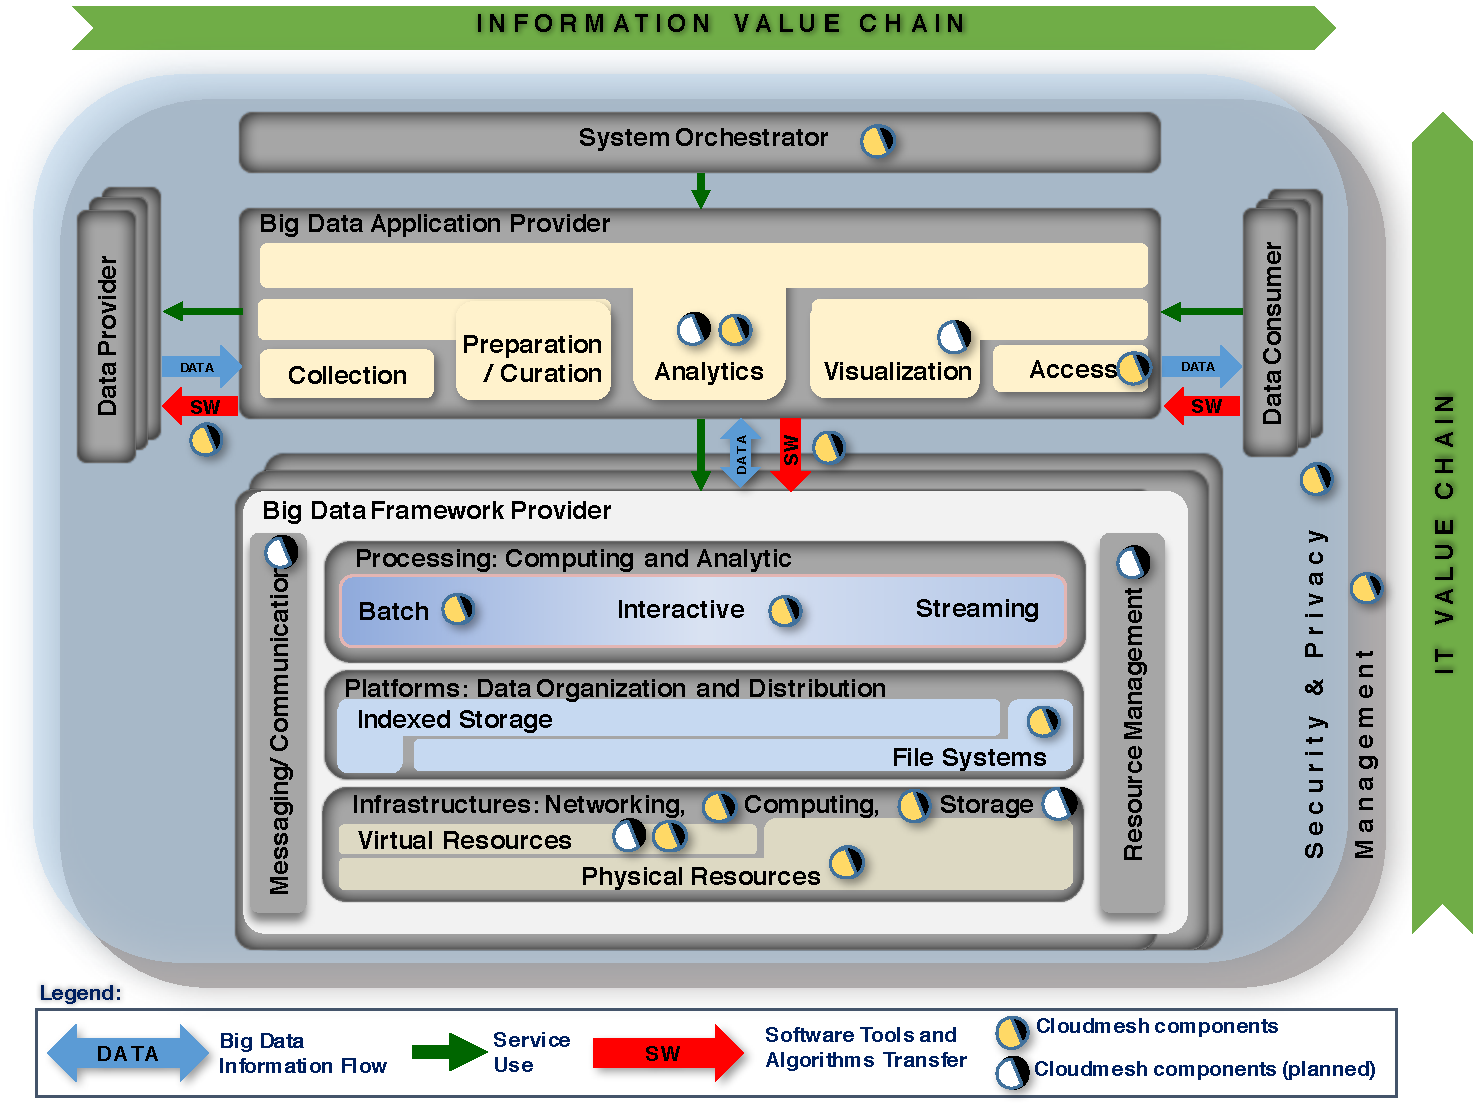
\includegraphics[width=1.0\columnwidth]{images/nist-bda.pdf}
  \caption{NIST Big Data Reference Architecture Diagram} 
  \label{F:NIST-arch}
\end{figure}


\begin{figure}[htb]
  \centering
     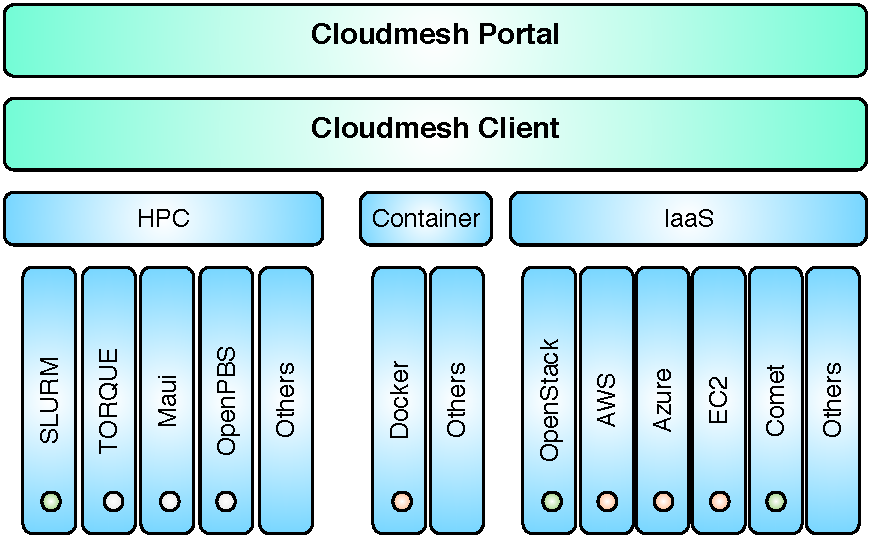
\includegraphics[width=1.0\columnwidth]{images/cloudmesh-arch-1.pdf}
  \caption{Cloudmesh layered Architecture} 
  \label{F:NIST-arch}
\end{figure}

\begin{figure}[htb]
  \centering
      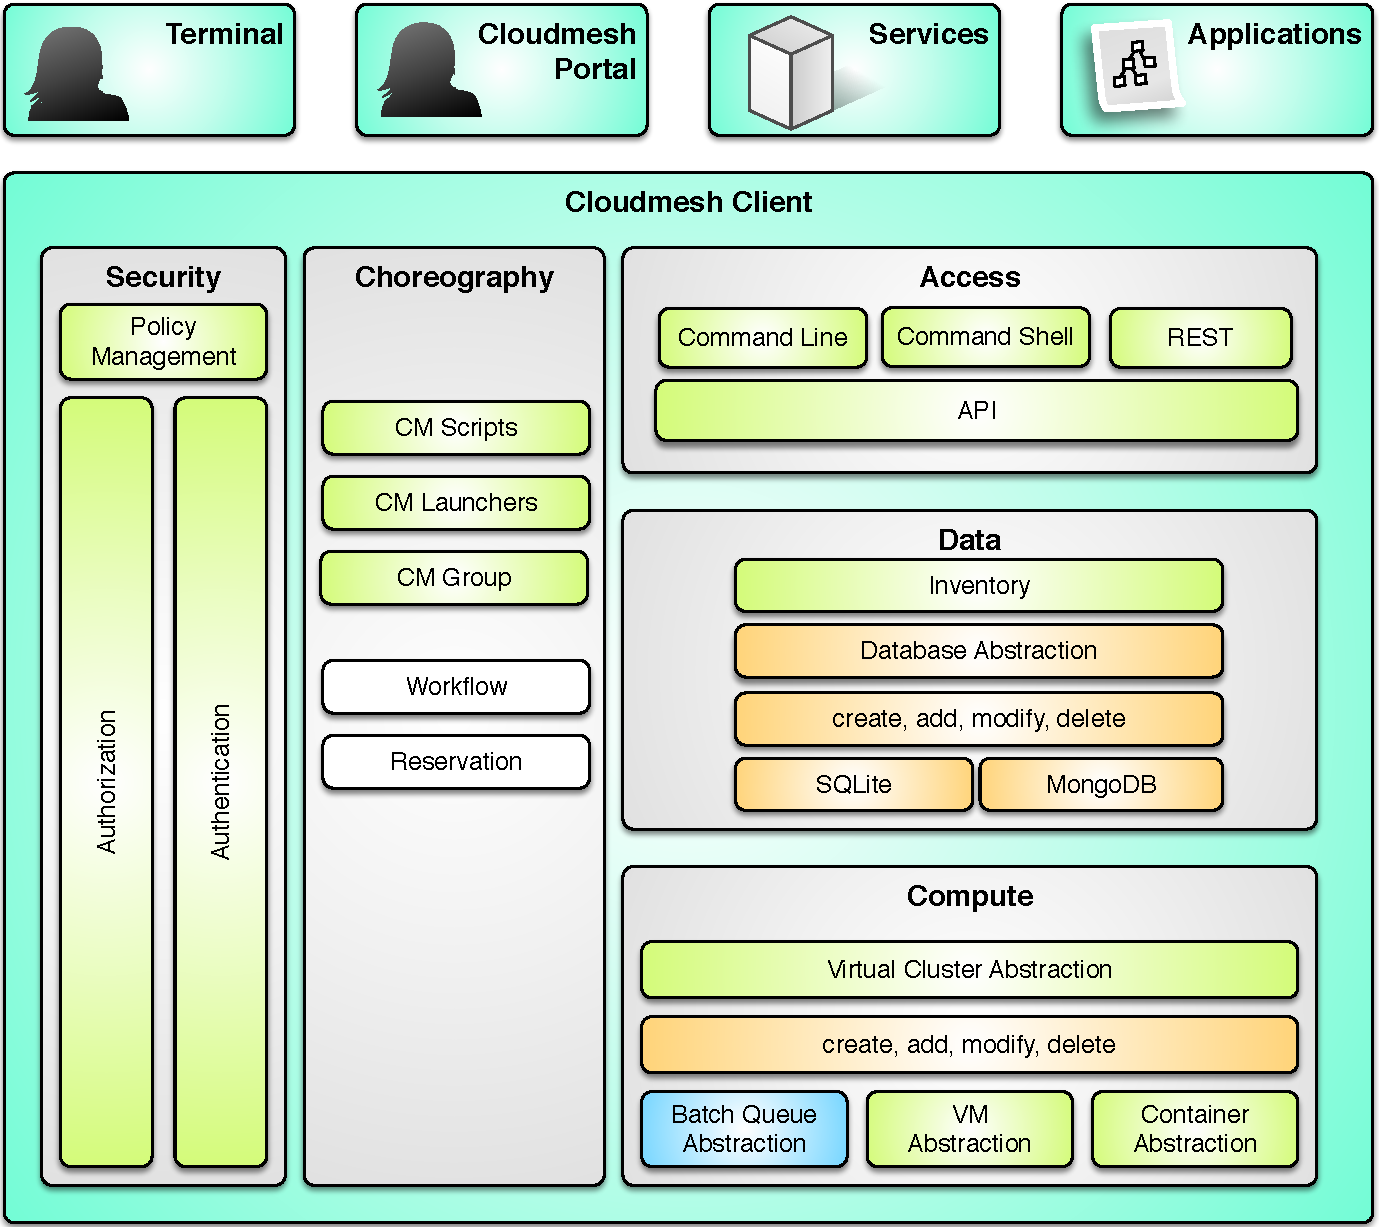
\includegraphics[width=1.0\columnwidth]{images/cloudmesh-arch-2.pdf}
  \caption{Cloudmesh components} 
  \label{F:NIST-arch}
\end{figure}

\begin{figure}[htb]
  \centering
      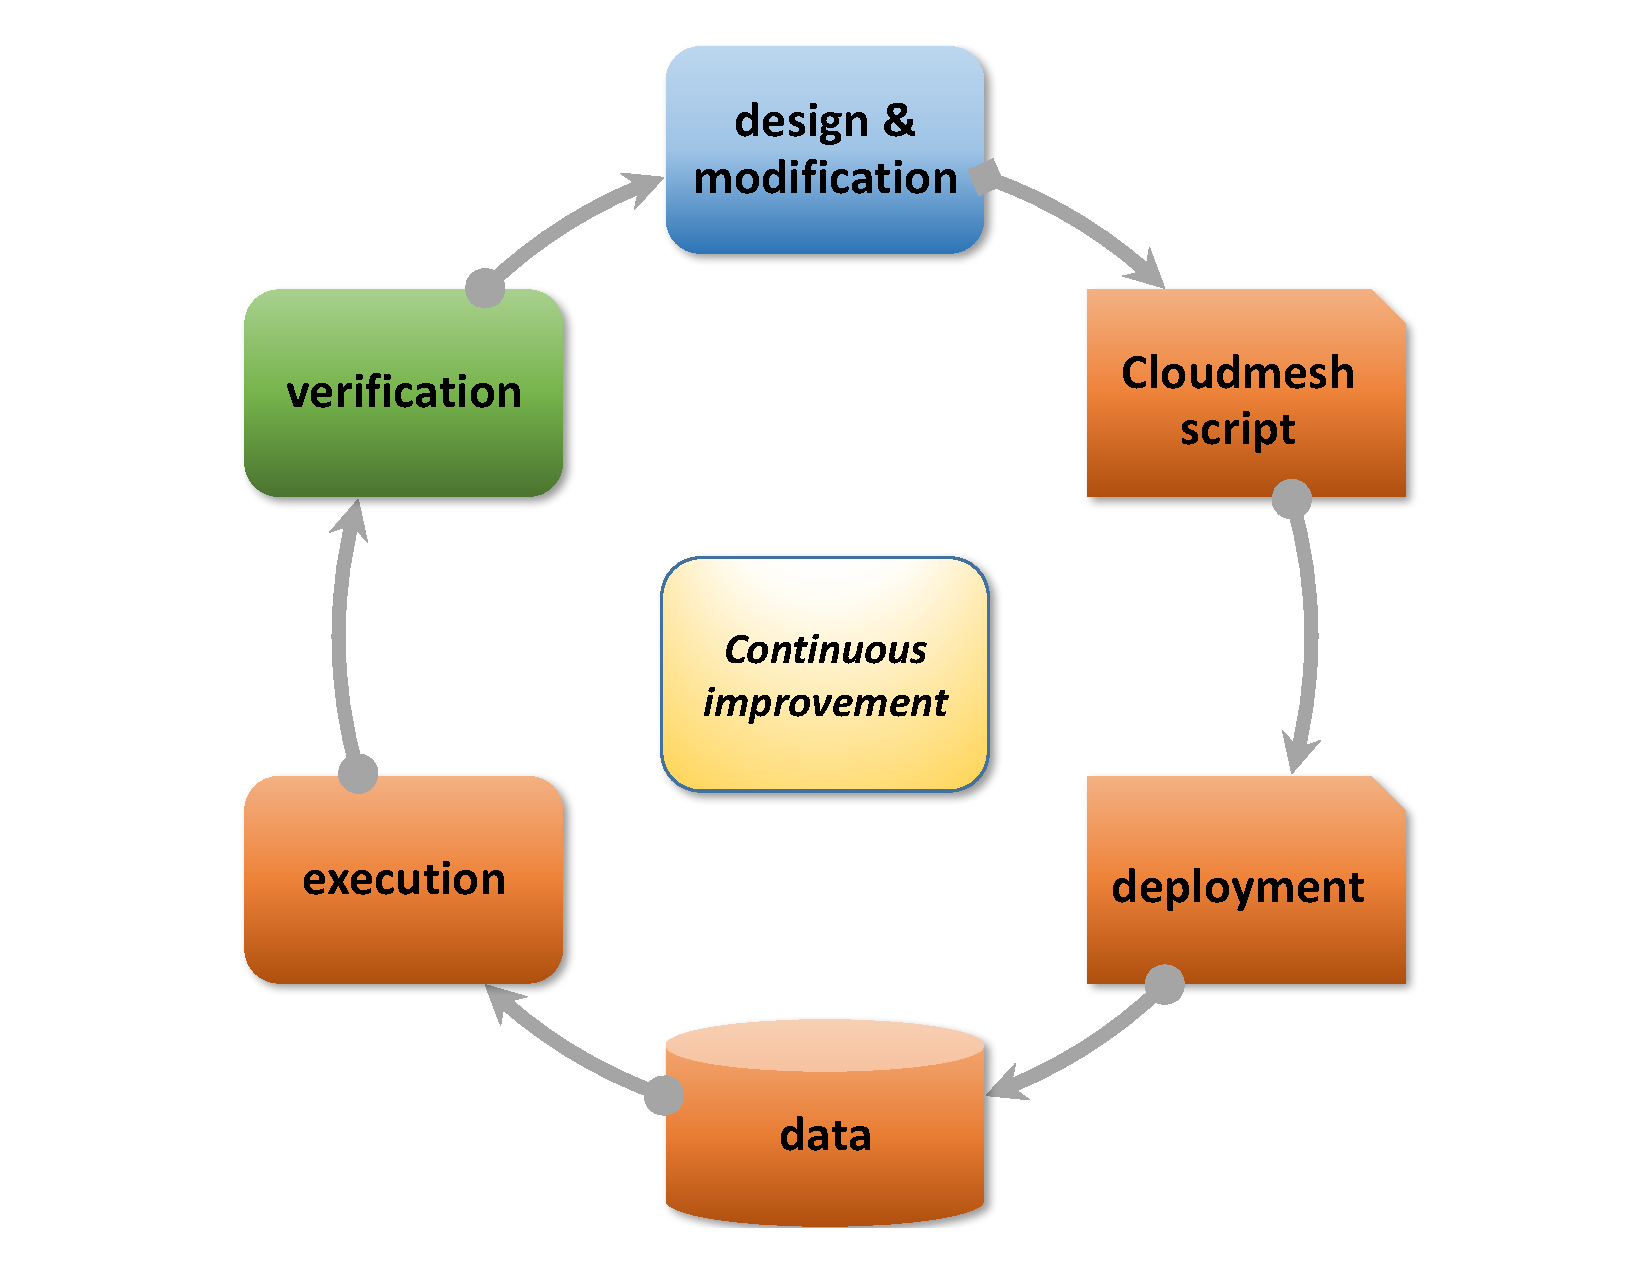
\includegraphics[width=1.0\columnwidth]{images/nist-devops-1.pdf}
  \caption{CM 1}
  \label{F:NIST-arch}
\end{figure}

\begin{figure}[htb]
  \centering
      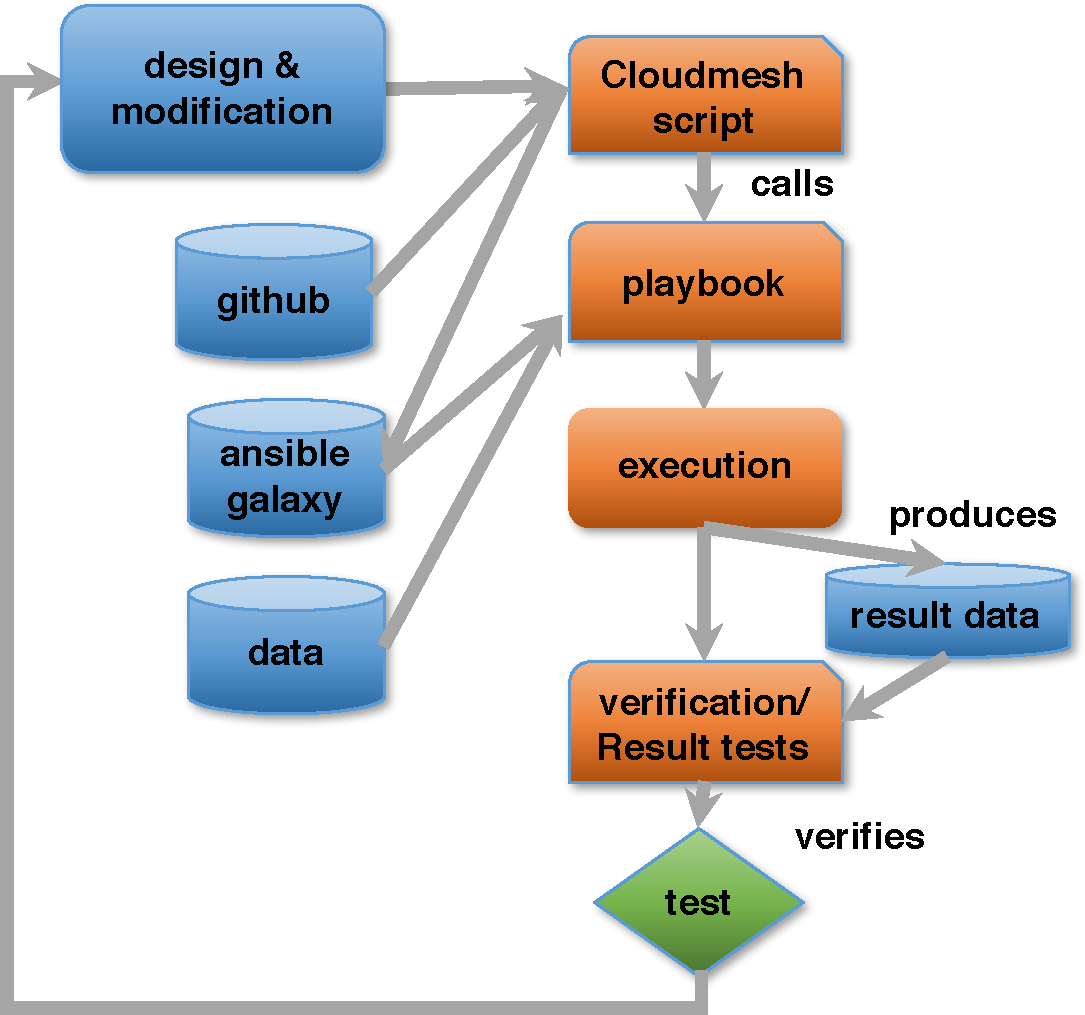
\includegraphics[width=1.0\columnwidth]{images/nist-devops-2.pdf}
  \caption{CM 2}
  \label{F:NIST-arch}
\end{figure}



It contains according to \cite{nist-bd} the following components:

\begin{description}

\item  {\bf System Orchestrator (or data scientist)} - provides high-level 
design dataflow between analytics tools and given datasets, computing system requirements, 
monitoring system resource and performance.


\item {\bf Data Provider} - provides abstraction of various types of 
data sources (such as raw data or data previously transformed by another system) 
and makes them available through different functional interfaces. This includes 
transfer analytics codes to data sources for effective analytic processing.


\item {\bf Big Data Application Provider} - provides analytics processing 
throughout the data lifecycle - acquisition, curation, analysis, visualization, 
and access - to meet requirements established by the System Orchestrator.


\item {\bf Big Data Framework Provider} - provides one or more instances 
of computing environment to support general Big Data tools, distributed file systems, 
and computing infrastructure - to meet requirements established by the Big Data 
Application Provider.


\item  {\bf Data Consumer} - provides interface to receive the value output 
from this NBD-RA ecosystem.


\item  {\bf Security and Privacy Fabric} - provides System Orchestrator 
the security and privacy interaction to the rest of the NBD-RA components to ensure 
protection of data and their content.


\item {\bf Management Fabric} - provides System Orchestrator the management 
interaction to the rest of the NBD-RA components with versatile system and software 
provisioning, resource and performance monitoring, while maintaining a high level 
of data quality and secure accessibility.

\end{description}


The focus of this document is on the Big Data Application Provider for how Big 
Data analytics can be applied/performed at each of its subcomponents. For the given 
mass amount of complex data, the process may involve one or more machine learning 
or analytic processing techniques at each of the subcomponents. 



\section{Cloudmesh Client}


The cloudmesh client toolkit is a lightweight client interface of
accessing heterogeneous clouds, clusters, and workstations right from
the users computer. The user can manage his own set of resources he
would like to utilize. Thus the user has the freedom to customize
their cyber infrastructure they use. Cloudmesh client includes an API,
a commandline client, and a commandline shell. It strives to abstract
backends to databases that are used to manage the workflow utilizing
the different infrastructure and also the services. Switching for
example to stage virtual machines from openstack clouds to amazon is
as simple as specifying the name of the cloud. Moreover, cloudmesh
client can be installed on Linux, MacOSX, and even Windows. Currently
we support backends to SLURM, SSH, Openstack, Heat. In the past we
supported AWS and Azure. We are in the process of integrating them
back into the client.


Cloudmesh client allows to easily manage virtual machines, containers,
HPC tasks, through a convenient client and API. Hence cloudmesh is not
only a multi-cloud, but a multi-hpc environment that allows also to
use container technologies (under development).

\begin{description}

\item{\bf Client based.} Cloudmesh client as the name indicates is a
client based toolkit that is installed and run on the users
computers. This also includes an add on component to the cloudmesh
client which is a portal. Hence we distinguish the client that
contains most of the functionality, as well as a portal that can
access the functionality through a locally maintaine Web
portal. Important to note is that the user manages its own credentials
and thus security and credential management is done directly on the
users machine instead through a hosted Web portal. This increases the
security as access to any credential is managed by the user and is not
part of a credential management system.

\item{\bf Layered Architecture.} Cloudmesh client has a layered
architecture that allows easy development of new features. This also
allows contribution by the community while developing integrated and
smaller sub components. Figure A depicts the various layers. A
resource abstraction layer allows the integration of a multitude of
resources spanning HPC, Containers, and Cloud resources. (At this time
we focus on Openstack and Slurm resources. We are working on
reintegrating resources such as Azure, AWS, Maui, Moab, and others
which we previously supported, as well as new resources such as
docker).

\item{\bf Management Framework.} Cloudmesh client contains a
management framework, and its components are depicted in Figure
B. cloudmesh allows easy management of virtual machines, containers,
and the data associated with them. We are currently developing a
choreography framework that leverages Ansible, chef, and heat. All of
the functionality is easily usable through a command shell that also
can be used from the command line, and a Python API. IN future we will
be providing a REST API.

\item{\bf Database Agnostic.} Cloudmesh contains some state about the
resource and environment that a user may want to use. The information
is managed in an database abstraction that would allow storing the
data in a variety of databases such as SQL and MongoDB. At this time
we have chosen SQLite to be the default database as it does not
require any additional setup and is universally available on all
operating systems without change.

\item{\bf Command shell and line.} Cloudmesh contains a command shell
allowing scripts to be developed and run. However we designed the
command shell in such a way that each command can also be called from
the command line. Through the cloudmesh state machine the state
between command shell, command client, and the portal is shared.

\item{\bf Cloudmesh Client Portal.} Previously, we distributed
cloudmesh with client, server, and a portal components in one
package. This however turned out to be to complex to be installed for
some of our less technically skilled user community. Thus we split up
the install into two independent packages. The cloudmesh client and
the cloudmesh portal. The portal provides some elementary features to
manage virtual machines and HPC jobs. At this time the portal is
considered to be alpha technology. Just as the client the portal is to
be run on the local user machine in oredr to allow increased security
by managing the credentials locally rather than on a server.

\item{\bf Cloudmesh Two Factor Authentication.} We have an
exploratory project in place that looks at the use of Yubikeys for
cloudmesh, client and cloudmesh portal.

\item{\bf Cloudmesh Comet.} We are actively developing the client
interface for SDSC’s comet supercomputer allowing bare metal
provisioning. The interface reuses cloudmesh components and
technologies while interfacing with the comet cloud REST
interface. The goal here is to manage virtual clusters.

\end{description}

\section{DESIGN}



\subsection{Goals}


<Goals statement> 

technology agnostic
easy to use
expandable
comprehensive


\subsection{Approach}



<Approach description>


\section{Selected Cloudmesh Components}

\subsection{cm hpc run SCRIPT}

submits the script to the cluster. The script will be copied prior to
execution into the home directory on the remote machine. If a DIR is
specified it will be copied into that dir.  The name of the script is
either specified in the script itself, or if not the default naming
scheme of cloudmesh is used using the same index incremented name as
in vms fro clouds: cloudmes husername-index



\begin{table*}[htb]
\caption{Selected Service Description}
\begin{center}
\begin{tabular}{|p{8cm}|p{9cm}|}
\hline
\blue \textbf{URL} & \blue \textbf{Description}\tabularnewline
\hline
\multicolumn{2}{|l|}{\grey\bf Virtual Cluster} \tabularnewline
\hline
cluster/list & TBD \tabularnewline
\hline
cluster/delete?id=<id> & TBD \tabularnewline
\hline
cluster/status?id=<id> & TBD \tabularnewline
\hline
cluster/create?provider=<provider> & TBD \tabularnewline
\hline
\multicolumn{2}{|l|}{\grey\bf Stack} \tabularnewline
\hline
stack/delete?id=<id> & TBD \tabularnewline
\hline
stack/status?id=<id> & TBD \tabularnewline
\hline
stack/create?cluster=<cluster> & TBD \tabularnewline

\hline
\multicolumn{2}{|l|}{\grey\bf Batch Experiments} \tabularnewline
\hline
hpc/run?script=<scriptname>\&cluster=<clustername>& submits an experiment to the named
                               cluster and returns the unique hpc
                               experiment id\tabularnewline
\hline
hpc/status?id=<id> & returns the status of the job started with the run
                  command \tabularnewline
\hline
hpc/delete?id=<id> & deletes the experiment with the given id\tabularnewline
\hline
 hpc/list & list all jobs started with the run command \tabularnewline
\hline
\end{tabular}
\end{center}
\end{table*}


\subsection{Implementation}

When developing solutions and examples for this book, I used the software and programming 
environments listed in Table~P-3.

\begin{table}[htb]
\caption{Software/programming environments}
\begin{center}
\begin{tabular}{|l|l|}
\hline
\textbf{Software} & \textbf{Version}\tabularnewline
\hline
Python &2.7.12\tabularnewline
\hline
Ansible & 2.3 \tabularnewline
\hline
Operating system& Linux, OSX, (Windows)\tabularnewline
\hline
Cloudmesh client &  4.3.7 \tabularnewline
\hline
\end{tabular}
\end{center}
\end{table}

All programs in this book were tested with Java/JDK7, Hadoop 2.5.0, and Spark (1.1.0, 
1.3.0, 1.4.0). Examples are given in mixed operating system environments (Linux 
and OS X). For all examples and solutions, I engaged basic text editors (such as 
vi, vim, and TextWrangler) and compiled them using the Java command-line compiler 
(javac).


In this book, shell scripts (such as bash scripts) are used to run sample MapReduce/Hadoop 
and Spark programs. Lines that begin with a \$ or \# character indicate that the 
commands must be entered at a terminal prompt (such as bash).

\section{Stack}


Big Data Stack
Introduction
The Big Data Stack (BDS) tackles the problem of reproducibly deploying a stack of software packages that need to be coordinated for analyzing Big Data. Given a cluster of machines, BDS deploys and configures a user-defined subset of the available modules. A number of modules are available (e.g. Apache Spark, Apache Drill) that the user can use to customize the cluster environment. The ultimate goal is to minimize the amount of work and complexity required to obtain a functional stack for big data analytics.

BDS was initially developed to aid students in completing data analytics projects. Consistently students would want to use various technologies and would get stuck during the installation and configuration phase, unable to progress. Since this inception, BDS has been adapted to be used in other scenarios, such as developing use cases for the study of Big Data projects.

BDS is available online at https://github.com/futuresystems/big-data-stack
Terms and Definitions
Big Data: data sets too large to fit on a single machine or whose analysis is infeasible on a single machine, required a large cluster of networked computers.
BDS: Big Data Stack
Role: an Ansible Role
Playbook: an Ansible Playbook
Module: a standalone deployment of a service for BDS defined as a playbook
Usage
Requirements: Git, Python 2.7, Ansible, SSH, IP addresses of the cluster machines

Assumptions for below:
The repository has been cloned and the current working directory is located inside the local copy
The IP addresses are accessible via ssh
The cluster is running Ubuntu 14.04 and as a user ubuntu with sudo privileges
The IP addresses are given in the shell variables $IP1, $IP2, $IP3, and $IP4

The first step is to define the cluster. This step assigns labels that will be used during deployment and configuration to subsets of the machines in the cluster

\begin{Verbatim}[fontfamily=helvetica]
$ ./mk-inventory -n mycluster $IP1 $IP2 $IP3 $IP4 \
                            > inventory.txt
\end{Verbatim}

The second step is to deploy Hadoop as this a requirement for installing the modules:

\begin{Verbatim}[fontfamily=helvetica]
$ ansibile-playbook play-hadoop.yml
\end{Verbatim}

Next, a subset of the modules (found in the addons directory) can be deployed:

\begin{Verbatim}[fontfamily=helvetica]
$ ansible-playbook addons/spark.yml addons/hive.yml \
                               addons/drill.yml
\end{Verbatim}

At this point Hadoop, Apache Spark, Apache Hive, and Apache Drill will have been installed and configured for use. The user may now log into the cluster and begin useing these tools.


\subsection{Use Case: Fingerprint Matching}

\subsection{Deployment Tools}
This section describes various deployment tools and approaches

\paragraph{SSH+Scripts}
\paragraph{Ansible}
\paragraph{Chef}
\paragraph{Puppet}
\paragraph{Salt}

\subsection{Defining Modules}
A BDS module is a playbook 

\subsection{Defining Roles}

\begin{Verbatim}[fontfamily=helvetica]
stack check [--stack=bds]
stack init [--no-activate] [--branch=master] [--user=$USER] 
               [--name=<project>] <ip>...
stack list [--sort=<field=date>] [--list=<field,...=all>] [--json]
stack project [<name>]
stack deploy [<play>...] [--define=<define>...]

Options:
   --format=FORMAT  the output format [default: table]
   --cloud=CLOUD    the cloud name
\end{Verbatim}

\subsubsection{Example}

The following example assumes that a cluster (Ubuntu
14.04) has been launched already and can be accessed by
the 'ubuntu` user at addresses 10.0.0.10, 10.0.0.11, and
10.0.0.12.


\begin{Verbatim}[fontfamily=helvetica]
cm stack check
\end{Verbatim}
verify the environment


\begin{Verbatim}[fontfamily=helvetica]
cm stack init --user ubuntu 10.0.0.10 10.0.0.11 10.0.0.12
\end{Verbatim}

create a project for the cluster with given username and addresses


\begin{Verbatim}[fontfamily=helvetica]

\end{Verbatim}

\begin{Verbatim}[fontfamily=helvetica]

\end{Verbatim}

\begin{Verbatim}[fontfamily=helvetica]
cm stack project
\end{Verbatim}

get the name of the project

\begin{Verbatim}[fontfamily=helvetica]
cm stack deploy play-hadoop.yml addons/spark.yml addons/hbase.yml
\end{Verbatim}

deploy hadoop, spark, and hbase to the cluster

\section{Use Cases}


\section{51 NIST Benchmarking Examples for Big Data}

\begin{description}

\item[Government Operation:] National Archives and Records
  Administration, Census Bureau

\item[Commercial:] Finance in Cloud, Cloud Backup, Mendeley
  (Citations), Netflix, Web Search, Digital Materials, Cargo shipping
  (as in UPS)

\item[Defense:] Sensors, Image surveillance, Situation Assessment
  Healthcare

\item[Life Sciences:] Medical records, Graph and Probabilistic
  analysis, Pathology, Bioimaging, Genomics, Epidemiology, People
  Activity models, BiodiversityDeep Learning and Social Media: Driving
  Car, Geolocate images/cameras, Twitter, Crowd Sourcing, Network
  Science, NIST benchmark datasets

\item[The Ecosystem for Research:] Metadata, Collaboration, Language
  Translation, Light source experiments

\item[Astronomy and Physics:] Sky Surveys compared to simulation,
  Large Hadron Collider at CERN, Belle Accelerator II in JapanEarth,

\item[Environmental and Polar Science:] Radar Scattering in
  Atmosphere, Earthquake, Ocean, Earth Observation, Ice sheet Radar
  scattering, Earth radar mapping, Climate simulation datasets,
  Atmospheric turbulence identification, Subsurface Biogeochemistry
  (microbes to watersheds), AmeriFlux and FLUXNET gas sensors

\item[Energy:] Smart grid

\end{description}

\begin{table*}[htb]

\caption{table of usecases}
\label{T:usecases}

TABLE COME HERE

\end{table*}


\section{Conclusion}

<Description> 

\subsection{Lessons Learned}

<General description>

\subsection{Future Works}


<General description>

\documentclass{article}
\usepackage{csvsimple}
\usepackage{longtable}
\usepackage{lscape}
\usepackage{array,graphicx}
\usepackage{booktabs}
\usepackage{pifont}
\usepackage{geometry}

\newcommand*\rot{\rotatebox{90}}
\newcommand*\OK{\ding{51}}
\newcolumntype{L}{>{\centering\arraybackslash}m{4cm}}

\begin{filecontents*}{list_of_projects_with_roles.csv}
ID,Use Case,Source,Hadoop,Mesos,Spark,Storm,Pig,Hive,Drill,HDFS,HBase,Mysql,MongoDB,RethinkDB,Mahout,D3 and Tableau,nltk,MLlib,Lucene/Solr,OpenCV,Python,Java,maven,Ganglia,Nagios,spark supervisord,zookeeper,AlchemyAPI,R,dataset,dataset size (GB)
 U.N1,NIST Fingerprint Matching,NIST,*,,*,,,*,*,,*,*,,,,,,,,,,*,*,*,*,*,*,,,Special Database 14 - NIST Mated Fingerprint Card Pairs 2.,2.1
 U.N2,Human and Face Detection,NIST,,*,*,,,,,,,,,,,,,,,*,*,,, ,,,*,,,INRIA Person Dataset,0.96
 U.N3,Twitter Analysis,NIST,,,,*,,,,,*,,*,,,*,*,,,,*,*,,,,,*,*,*,Twitter,
 U.N4,Analytics for Healthcare Data/Health Informatics,NIST,*,,*,,,,,,*,,,,*,*,,*,*,,,*,, ,,,*,,,Medicare Part-B in 2014 from Center for Medicare and Medicaid Services (CMS),0.1
 U.N5,Spatial Big Data/Spatial Statistics/Geographic Information Systems,NIST,*,,*,,,,,,,,,,*,*,,*,,,,*,*,,,,,,,Uber,0.2
 U.N6,Data Warehousing and Data Mining,NIST,*,,*,,*,*,,,*,,*,,*,*,,*,*,,,*,,,,,*,,,,count,,,,4,1,5,1,1,2,1,0,4,1,2,0,3,4,1,3,2,1,2,5,2,3,1,1,5,1,1,,
 \end{filecontents*}

\begin{document}

\newgeometry{margin=1cm}
\begin{table} \centering
  \begin{tabular}{@{} cl*{26}c @{}}
    & ID & \rot{Hadoop} & \rot{Mesos} & \rot{Spark} & \rot{Storm} & \rot{Pig} & \rot{Hive} & \rot{Drill} & \rot{HDFS} & \rot{HBase} & \rot{Mysql} & \rot{MongoDB} & \rot{RethinkDB} & \rot{Mahout} & \rot{D3 and Tableau} & \rot{nltk} & \rot{MLlib} & \rot{Lucene/Solr} & \rot{OpenCV} & \rot{Python} & \rot{Java} & \rot{Ganglia} & \rot{Nagios} & \rot{zookeeper} & \rot{AlchemyAPI} & \rot{R} & \rot{\shortstack{dataset\\ size (GB)}} \\
    \hline
    & U.N1 & \OK &  & \OK &  &  & \OK & \OK &  & \OK & \OK &  &  &  &  &  &  &  &  &  & \OK & \OK & \OK & \OK &  &  & 2.1 \\
    \hline
    & U.N2 &  & \OK & \OK &  &  &  &  &  &  &  &  &  &  &  &  &  &  & \OK & \OK &  &   &  & \OK &  &  & 0.96 \\
    \hline
    & U.N3 &  &  &  & \OK &  &  &  &  & \OK &  & \OK &  &  & \OK & \OK &  &  &  & \OK & \OK &  &  & \OK & \OK & \OK \\
    \hline
    & U.N4 & \OK &  & \OK &  &  &  &  &  & \OK &  &  &  & \OK & \OK &  & \OK & \OK &  &  & \OK &   &  & \OK &  &  & 0.1 \\
    \hline
    & U.N5 & \OK &  & \OK &  &  &  &  &  &  &  &  &  & \OK & \OK &  & \OK &  &  &  & \OK &  &  &  &  &  & 0.2 \\
    \hline
    & U.N6 & \OK &  & \OK &  & \OK & \OK &  &  & \OK &  & \OK &  & \OK & \OK &  & \OK & \OK &  &  & \OK &  &  & \OK &  &   \\

  \end{tabular}
 \end{table}

 \begin{tabular}{l|l|l|L}%
   \bfseries ID& \bfseries Use Case & \bfseries Source & \bfseries Dataset% specify table head
   \csvreader[head to column names]{list_of_projects_with_roles.csv}{}% use head of csv as column names
   {\\\hline\ID &\csvcolii &\Source &\dataset}% specify your coloumns here
 \end{tabular}

 \restoregeometry
\end{document}





\section{Background}

\subsection{Deployment}

Big Data Software Stack is built with various software packages from different layers (and it’s increasing), therefore accomplishing these multiple software deployment is challenging
\subsection{Documentation}
installation and configuration steps should be documented in every particular to guarantee successful deployment
\subsection{Repeatable and Automated Deployment}
Same results are expected by offering repeatable deployments when a new system is built
Potentially targeting different infrastructures via virtual clusters
\subsection{Cross-Platform Configuration}
It ensures working, executable software deployment on multiple platforms, distributions and versions
DevOps can be used to support this workflow


\section{Ansible}

\subsection{Overlap of Technologies}
6 projects from the 51 NIST use cases
81 other projects surveyed as part of classes taught at Indiana University
Findings
We found 62 roles(*) from which many are repeatedly used in various projects. 
We have chosen Ansible to implement the deployment descriptions because 

(*) we will define later what a role is

\subsection{Why Ansible?}
Expandable: Leverages Python (default) but modules can be written in any language
Simplicity: 
Agentless: no setup required on managed node
Security: Allows deployment from user space; uses ssh for authentication
Flexibility: only requires ssh access to privileged user
Transparency: YAML Based script files express the steps of installing and configuring software
Modularity: Single Ansible Role (should) contain all required commands and variables to deploy software package independently
Sharing and portability: roles are available from source (github, bitbucket, gitlab, etc) or the Ansible Galaxy portal

\subsection{Ansible for NIST deployments}
6 NIST examples
19 roles for Fingerprint 
5 roles for Face detection 
27 roles for the other four NIST use cases
Twitter Analysis
Analytics for Healthcare Data/Health Informatics
Spatial Big Data/Spatial Statistics/Geographic Information Systems
Data Warehousing and Data Mining
36 Projects from class, Spring '16 
41 roles
45 Projects from class, Fall '15
62 roles, 39 datasets

\subsection{Relationship between Roles and Projects}
\subsection{Features of Ansible fostering reproducibility}
Ansible provides a structured environment for defined sets of tasks to execute on a number of nodes. Tasks are ideally idempotent.
There are two basic methods for organizing tasks:
Playbooks: main entry points, specific to environments
Roles: reusable abstraction (analogous to functions)
Playbooks provide the primary entry point, and consist of tasks that are either defined directly in the playbook, or externally via roles.
Roles are groups of related tasks that can be distributed and reused independently of playbooks.
The Inventory file identifies the nodes controlled by Ansible.
\subsection{Using Roles and Playbooks: Face Detection Example }


\subsection{Ansible: Inventory, IaaS, PaaS}
The inventory file for Ansible groups the IP addresses of the infrastructure into named sets.
On the right are two examples of inventory files:
Top: a static inventory for a cluster with two nodes in the "webservers" group and one node in the "databases" group.
Bottom: a dynamic inventory in which a script is called to define the nodes. The output must be specifically-formatted JSON for Ansible.
\begin{Verbatim}
[webservers]
10.0.0.1
10.0.0.2
[databases]
10.0.0.3
#!/use/bin/env bash

python dynamic-nodes-setup.py
\end{Verbatim}

\subsection{Ansible: Roles}
Roles are primarily defined as a collection of related tasks to accomplish a single goal.  These tasks can be configured via variables, that may be overridden when the role is used in a playbook.
On the top right is an example directory structure defining a role for Apache Spark: Tasks are defined in the tasks/main.yml file, Variables are defined in defaults/main.yml
On bottom right is an elided set of the entries in tasks/main.yml. These tasks use the ``get\_url'', and ``unarchive'' modules and optionally builds from source when spark\_package\_type is "src"
\begin{Verbatim}
spark
- defaults
   - main.yml
- LICENSE
- README.md
- tasks
    - build.yml
    - main.yml
\end{Verbatim}

\begin{Verbatim}
---

- name: download
  get_url:
    url: "{{ spark_url }}"
    dest: "{{ ansible_env.PWD }}/{{ _spark_package_name }}"
    sha256sum: "{{ spark_sha256 }}"
  
- name: extract
  unarchive:
    dest: "{{ spark_install_dest }}"
    src: "{{ ansible_env.PWD }}/{{ _spark_package_name }}"
    copy: no
    creates: "{{ spark_install_dest }}/{{ _spark_directory }}"
  
- include: build.yml
  when: spark_package_type == 'src'

# ...

Ansible: Playbooks
An example playbook is shown to the right.

Name: description of this play

Hosts: the set of nodes on which to operate, named in the inventory file

Become: escalate privileges

Roles: list of roles to apply, with overridden variables as needed.
---

- name: install and configure spark
  hosts: frontendnodes
  become: yes
  roles:
    - role: java
    - role: maven
    - role: spark
      spark_version: 1.6.0
      spark_package_type: bin
\end{Verbatim}


\subsection{Ansible: Role Repositories}

There are two primary mechanisms available to redistribute roles

Ansible Galaxy is the primary hub for sharing roles. The
ansible-galaxy tool can install these roles. Useful for using
externally-developed roles

Directly from the source code repositories. In the case of using Git,
these repositories can be installed as git submodules. Useful for
internally-developed roles

We have found that installing roles as git submodules allows the
flexibility to both use roles developed elsewhere as well as make
modifications and even contribute those changes upstream.

\subsection{Ansible: Vetting Roles}
An important aspect of developing roles is the vetting step. In a
production environment, each role must be examined for security
vulnerabilities as well as to ensure that they will function as
expected. Externally-developed roles may need to be adapted to work in
the target environment. When a role is defined, variables to modify
the deployment behavior need to be exposed. We have found that many
roles made available only expose a subset of the application's
available configuration options and may not work outside the author's
environment.

Projects
List of Projects
27 roles are collected from 6 NIST use cases. Hadoop, Spark, HBase,
D3, Tableau, Java and Zookeeper are frequently reused more than four
out of six use cases.

Table 1. List of Projects with Roles

Table is in Google sheet: 
% \url{https://docs.google.com/spreadsheets/d/1idB11ibeITgTLUT9D_xT6cOMsVzdG2cVa3o0w_Wh7IE/edit?usp=sharing}

Roles from NIST and Class (Survey)


\section{Big Data Stack (BDS)}
BDS is a collection of playbooks for deploying the tools of big data analytics, given a set of accessible IP addresses. It allows the user to select a subset of the available tools to deploy in order to customize their virtual cluster.
Example: to setup a stack with Hadoop, Spark, and Hive:
$ ansible-playbook play-hadoop.yml addons/spark.yml addons/hive.yml
Example: to setup a stack with Hadoop, HBase, and Drill:
$ ansible-playbook play-hadoop.yml addons/hbase.yml addons/drill.yml
It is provided online at https://github.com/futuresystems/big-data-stack

Roles and playbooks offered by BDS        (as of 27 Sep., 2016)
Roles
Drill
Ganglia
Hadoop
Hbase
Hive
Java
Limits
Maven
Mysql
Nagios
Pig

Roles (cont.)
Spark
Supervisord
Zookeeper

Playbooks
Hadoop
Hbase
Pig
Spark
Drill
Hive


\subsection{Towards Cloudmesh}
BDS is ideally suited to be included in cloudmesh as one of its deployment management tools. Cloudmesh adds features to easily access infrastructure.
  … more in the next another section we present later

Examples
Face Detection Example
Example 1: Face Detection Lifecycle
\begin{Verbatim}
[masters]
10.0.0.1
10.0.0.2
10.0.0.3
[workers]
10.0.0.4
10.0.0.5
10.0.0.6
Example 1: Face Detection Lifecycle on AWS
[masters]
10.0.0.1
10.0.0.2
10.0.0.3
[workers]
10.0.0.4
10.0.0.5
10.0.0.6
u'tag_masters_True': [u'52.23.213.103', u'54.196.41.145',u'54.209.137.235'],
u'tag_workers_True': [u'52.23.213.104', u'54.196.41.146',u'54.209.137.237'], ...
\end{Verbatim}

Example 1: Face Detection Screenshot Running EC2 provisioning playbook
on command line:

\begin{Verbatim}
$ ansible-playbook boot-ec2-with-vpc.yml -i ec2.py
\end{Verbatim}

\section{Virtual Clusters}
\subsection{Motivation}
Traditional HPC provided clusters to the community. The clusters are managed by professional staff and have mostly rigid software stack.
Advantages: provides well defined environment to the community, provides often optimized services for this particular system or the community it serves, allows sharing of resources through queuing system
Disadvantages: Different communities, Groups or projects may have different requirements that are not met by the software stack, software stack often not state-of-the art, but tuned for reliability, experimentation with new software and methodologies in such an environment is difficult, queuing system may not provide enough interactivity
Can we build a more flexible environment
Support custom software stacks
Support different interaction modes with instantaneous access without wait time
Support the use of heterogeneous platforms to allow increase in availability as well as features
Support the easy management of such an environment

\subsection{Virtual Clusters}

Definition: A set of compute, storage and network services that
interact with each other to serve an application or community for a
specific amount of time to support one or more experiments. A virtual
cluster is managed by the community or application user. They are
typically built on top of HPC, Grids, Clouds, and Containers. The
virtual cluster is managed by the user.

Contrasting Grids: targeted towards the support of a virtual
organization introducing high overheads on the deployment and
management of such infrastructure. Grids are a natural expansion of
traditional supercomputer centers that are managed by professional
staff. Contrasting Cloud IaaS: offer typically low level IaaS services
allowing users to combine them. They are a valuable building block for
virtual clusters. Clouds are managed by professional staff.

Contrasting Cloud PaaS: offer enhanced services to users targeting a
particular platform. They are offered by professional staff.

Contrasting Containers: offer an abstraction to share the existing hardware and OS while using containers making the it not necessary to us OS virtualization, thus saving space. Containers provide very useful enhancements for creating virtual clusters through add ons such as Kubernetes and Docker Swarm.



\subsection{Cloudmesh Access and Management of virtual clusters}
Cloudmesh is an API, command line tool, and command shell allowing the easy utilization of HPC, Clouds, Containers through machine abstractions
Switching between alternative services can be achieved by updating a
single variable.

Demonstrated usages of
Comet                                                                                           (HPC integrated Cloud)
FutureSystems, Chameleon, CloudLab, Bridges, Jetstream, …  (National Openstack Clouds)
Cybera (CA), Karslruhe Openstack Cloud (KIT, Germany), …     (International)
EC2, AWS, Azure                                                                          (Commercial Non Openstack)
Devstack, Trystack, Virtualbox                                                       (Desktop Clouds)
A user could use all of them

\subsection{Cloudmesh and Comet Cloud Virtual Cluster}
Comet is a NSF sponsored super computer offered by SDSC to the community. It operates in two modes: HPC and virtual clusters
Comet virtual clusters are low level and offer the HPC administrator the view of a cluster as if it were hardware. This is achieved via virtualization and low level exposure of network services. The administrator has full control over the cluster.
This is achieved by the integration of virtualization and SRIOV within Rocks. Thus the same cluster can not only be used in virtualized mode, but also in HPC mode
Comet users can therefore use HPC and virtualized clusters on the same hardware. Virtual clusters are treated as a special kind of compute job
Based on our long experience in this field we have delivered to SDSC an extension to cloudmesh that allows the creation and management of virtual clusters within comet
We can today use more than Comet
Accessing Virtual Clusters
REST API
Command line interface
Command shell for scripting
Console Access
Web Page

\begin{Verbatim}
Simple commands allow easy management
cm comet cluster  ID
Show the cluster details
cm comet power on ID vm-ID -[0-3] --walltime=6h
Power 3 nodes on for 6 hours
cm comet image attach image.iso ID vm-ID-0
Attach an image
cm comet boot ID vm-ID-0
Boot node 0
cm comet console vc4
Console 

Switching infrastructure in cloudmesh is easy
cm var cloud=jetstream / bridges / aws / …
cm default cloud=$cloud
cm boot
\end{Verbatim}

\subsection{Cloudmesh Launcher abstraction}
Important is that cloudmesh introduces an abstraction for creating virtual clusters that we call “launcher”. A launch specifies the creation of a virtual cluster. Such a launch can use
Ansible
Chef, …
Openstack Heat
Ssh
Make
Pegasus (Grids)
Hence a variety of different launch platforms can be integrated into cloudmesh and work from different community contributions can be supported.

Building virtual clusters is easy
cm launcher cluster -n 10
Gives a virtual cluster with 10 nodes and allows the user to login between each node


cm launcher hadoop -n 10 --cloud=rackspace
Finds the playbook for creating a hadoop cluster and launches it on a cloud called rackspace



Building enhance virtual clusters is easy
Virtual cluster for face detection
cm launcher facedetection -n 10 --cloud=rackspace
Finds the playbook for creating a virtual cluster and launches the deployment for the face detection project.
Cloudmesh will look in the git repository to locate the ansible scripts and execute them


Cloudmesh Launcher Portal (in development)
       Specific Launch                                    List of Launchers





Automatically generates Graphical representation of input parameters                                  
\subsection{Conclusion}
Ansible + Cloudmesh
Will enable re-usable specification of Big Data Stack applications in 87 use cases and 62 unique roles from which NIST has 27
BDS status
From this a total part of BDS are vetted (the most fundamental ones): 
14 Roles  (about 50% done of NIST roles)
6   Playbooks

\subsection{Cloudmesh Status}
We can replicate on different infrastructures including AWS, Azure, Openstack, Comet …
We need to complete the launcher and integration of the BDS into the launcher




\end{document}
